\documentclass[10pt]{article}

\usepackage[letterpaper,left=0.5in,right=0.5in,top=1in,bottom=1in]{geometry}

\usepackage[T1]{fontenc}
\usepackage[utf8]{inputenc}
\usepackage{lmodern}

\usepackage[activate={true,nocompatibility},final,tracking=true,kerning=true,spacing=true,factor=1100,stretch=10,shrink=10]{microtype}
\microtypecontext{spacing=nonfrench}
\usepackage{xspace}
\usepackage{amssymb,amsfonts,amsmath}
\usepackage{lipsum,xcolor}
\usepackage{graphicx}
\usepackage{float,caption,subcaption,wrapfig}
\usepackage{tcolorbox}
\usepackage{listings}
\usepackage{courier}
\usepackage[english]{babel}
\usepackage{textcomp}
\usepackage{csquotes}
\usepackage{siunitx}
\usepackage[makeroom]{cancel}
\usepackage[shortlabels]{enumitem}
\sisetup{mode=text,
         group-separator={,},
         detect-all,
         binary-units,
         list-units = single,
         range-units = single,
         range-phrase = --,
         per-mode = symbol-or-fraction,
         list-final-separator = {, and }
}

\lstset{basicstyle=\ttfamily,
        breaklines=true,
        numbersep=-8pt,
        numberstyle=\small,
        numbers=right,
        frame = single, 
        showstringspaces=false,    
        keywordstyle=\color{blue}\bf,
        commentstyle=\color{darkgray},
        stringstyle=\color{purple}\bf,
  }

\DeclareSIUnit\atm{atm}
\DeclareSIUnit\bar{bar}

\headheight = 13.6pt
\usepackage{fancyhdr}
\pagestyle{fancy}

\lhead{PH 641 Sp2020}
\chead{Quiz 6}
\rhead{Due 5:00 pm, 23 April 2020}

\rfoot{Submitted by: Paige Lorson}
\tcbset{width=(\linewidth-2mm),before=,after=\hfill,colframe=black,colback=white,}
\newcommand{\volume}{{\ooalign{\hfil$\vol$\hfil\cr\kern0.08em--\hfil\cr}}}
\newenvironment{Solution}
    {\textbf{Solution:}
    
    \vspace{5mm}
    \begin{tcolorbox}
    }
    {
    \end{tcolorbox}
    \vspace{5mm}
    % \newpage
    }
\newcommand{\vol}{{\ooalign{\hfil$V$\hfil\cr\kern0.08em--\hfil\cr}}}
\renewcommand\labelitemi{$\cdot$}

\begin{document}

\noindent\textbf{Quiz problem 1:}  The van der Waals (vdW) equation
$$
\left(P+N^{2} a / V^{2}\right)(V-N b)=N k_{B} T
$$
is often applied as an approximate equation of state for real liquids and gases. The term $V-N b$ arises from short-range repulsion between molecules (Exercise 3.5 ); the term $N^{2} a / V^{2}$ incorporates the leading effects $^{20}$ of long-range attraction between molecules.

Figure 11.13 shows the val $W$ pressure versus volume curves for one mole of $\mathrm{H}_{2} \mathrm{O}$. Trace over the figure, or download a version from the book web site $[126] . \quad$By hand, roughly implement the
Maxwell construction for each curve, and sketch
the region in the $\overrightarrow{P-V}$ plane where liquid and gas can coexist.

\begin{Solution}\centering{
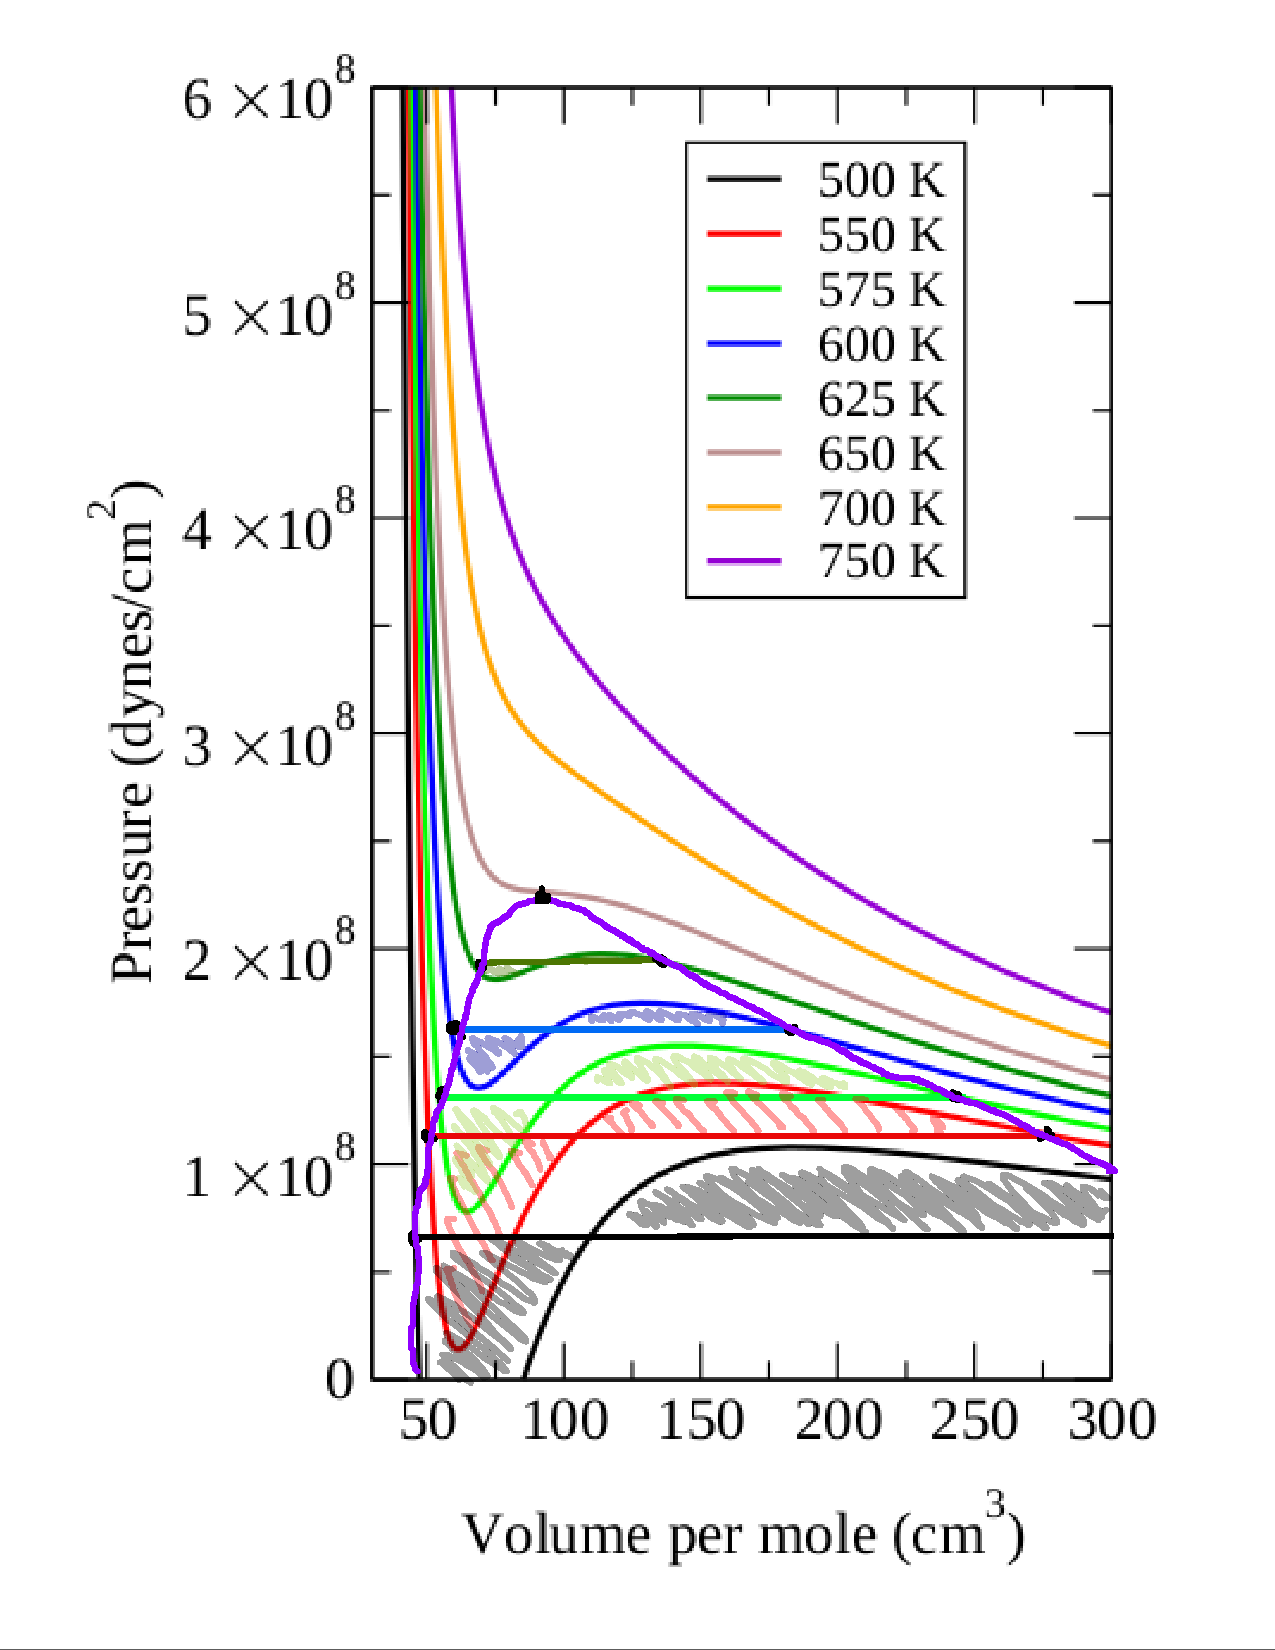
\includegraphics[width=4in]{Quizzes/dome_EOPC_fig11_13.pdf}}

\end{Solution}


\noindent\textbf{Quiz problem 2:} The top of the coexistence curve in Fig. 11.13 is the pressure, density, and temperature at which the distinction between liquid and gas disappears. It is the focus of much study, as the prime example of a critical point, with self-similar fluctuations and scaling behavior.
(a) Identify this point on a sketch of Fig. 11.13 The vdW constants are fit to the critical temperature $T_{c}=647.3 \mathrm{K}$ and pressure $P_{c} = 22.09 \mathrm{MPa}=220.9 \times 10^{6} \mathrm{dyne} / \mathrm{cm}^{2} ;$ check that
your estimate for the critical point roughly agrees with the values quoted. I have found few references that quote the critical volume per mole, and the two I have found disagree; one says around $50 \mathrm{cm}^{3} / \mathrm{mol}$ and one says around $55 .$ Plot the true critical point on your sketch. Is the location of the critical density of water predicted well by the vdW equation of state?

\begin{Solution}
\centering{
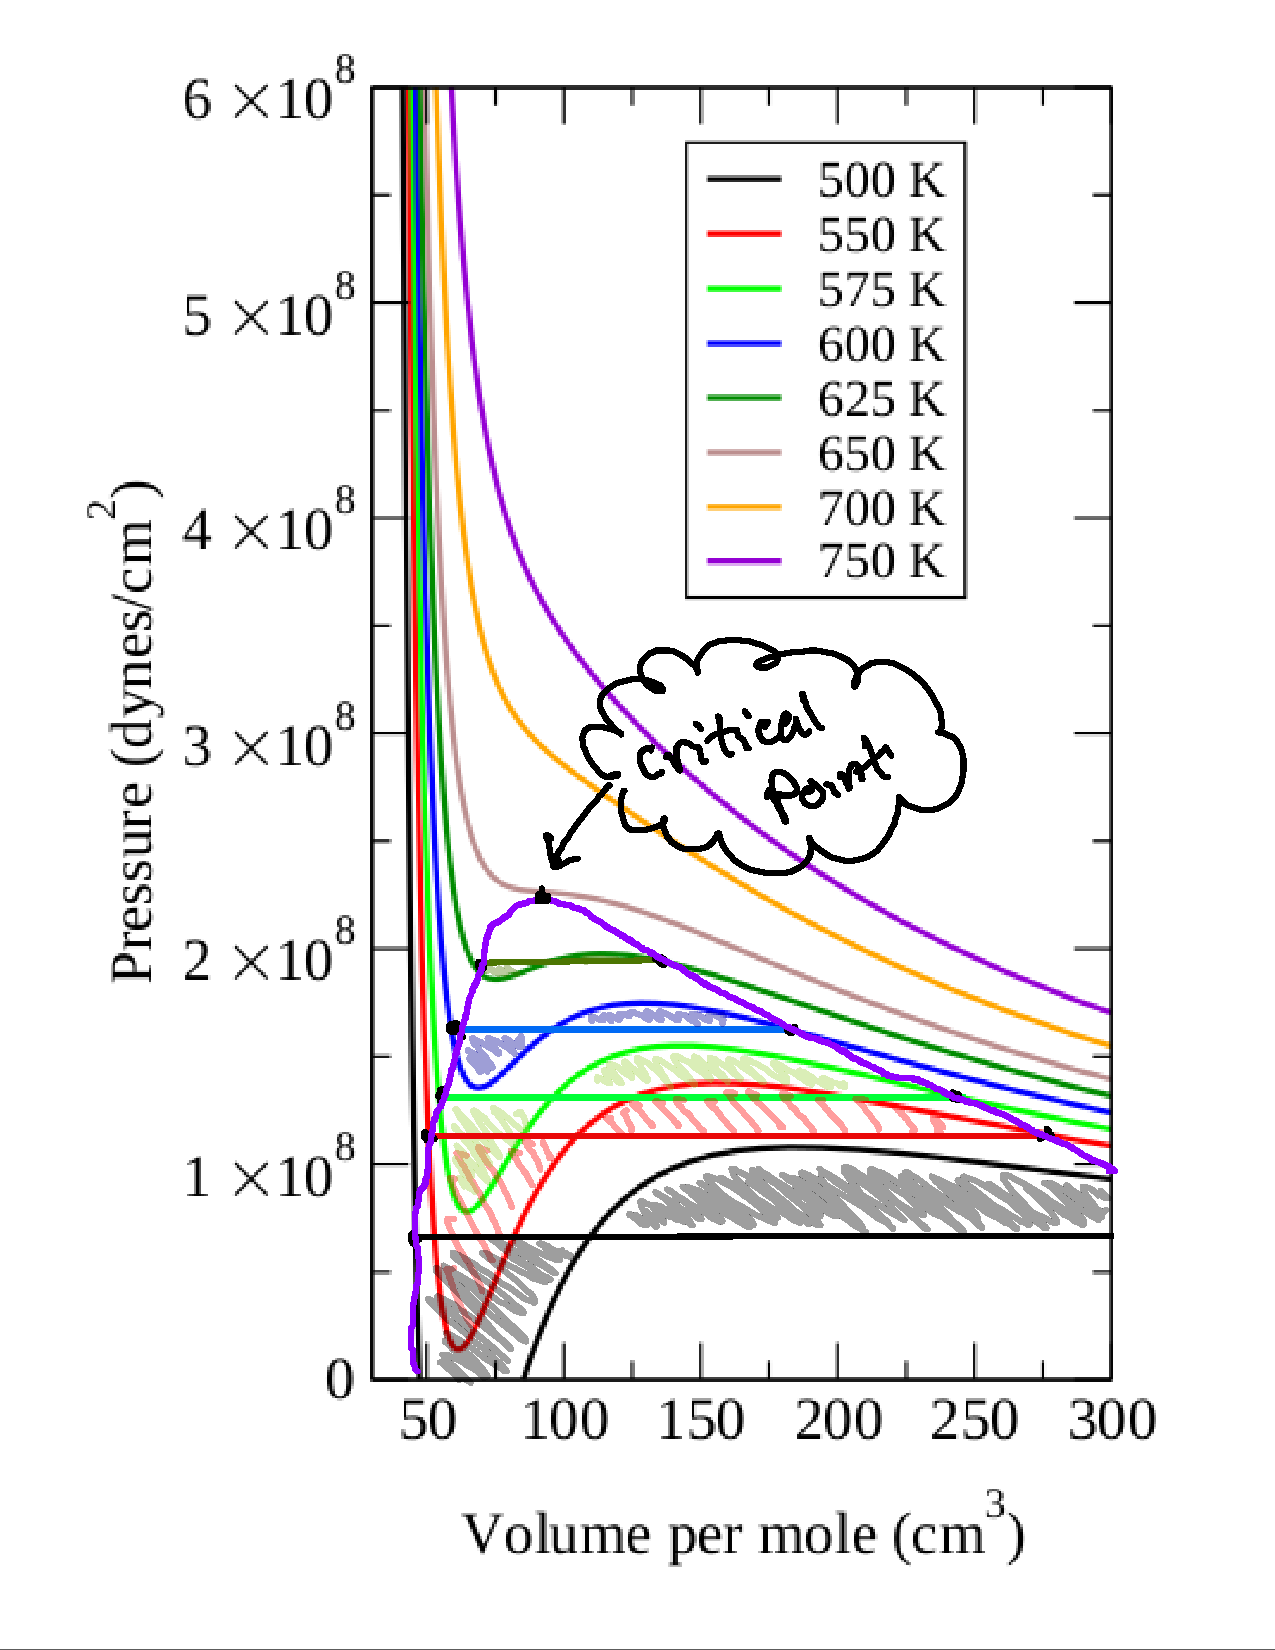
\includegraphics[width=4in]{Quizzes/critPt- EOPC_fig11_13.pdf}}
\end{Solution}

\end{document}